% Document setup----------------------------------------------------------------
\documentclass[10pt, xcolor=dvipsnames,compress]{beamer}
\usetheme{Berlin}

% Presentation setup------------------------------------------------------------
\setbeamertemplate{footline}[frame number] % Include page number
\beamertemplatenavigationsymbolsempty      % Remove navigation bar
\usecolortheme{metropolis}

\setbeamercolor{background canvas}{bg=white}
\setbeamercolor{titlelike}{bg=white}
\setbeamercolor{titlelike}{bg=white}
\setbeamercolor{author}{bg=white}
\setbeamercolor{institute}{bg=white}
\setbeamercolor{date}{bg=white}

% Title page in sections -------------------------------------------------------
\AtBeginSection[]{
  \begin{frame}
    \vfill
    \centering
    \begin{beamercolorbox}[sep=8pt,center,shadow=false,rounded=true]{title}
        \usebeamerfont{title}\insertsectionhead\par
    \end{beamercolorbox}
    \vfill
  \end{frame}
}

% Import packages---------------------------------------------------------------
% Aesthetics packages ----------------------------------------------------------
\usepackage{amsfonts}

% Aesthetic commands -----------------------------------------------------------
\definecolor{marineblue2}{rgb}{0.05,0.1,0.5}

% Math packages ----------------------------------------------------------------
\usepackage{amsmath}
\usepackage{bbm}

% Referencing packages ---------------------------------------------------------
\usepackage{hyperref}

% Math commands ----------------------------------------------------------------
\newcommand{\N}{\mathbb{N}}
\newcommand{\Z}{\mathbb{Z}}
\newcommand{\R}{\mathbb{R}}


% Define title -----------------------------------------------------------------
\title{P218 Econometrics I}
\subtitle{TA Session 0}
\author{Gabriel Simões Gaspar}
\institute{London Business School}
\date{Fall 2022}

% Start document ---------------------------------------------------------------
\begin{document}

% Title frame ------------------------------------------------------------------
\maketitle

% Outline frame ----------------------------------------------------------------
\begin{frame}{Roadmap}
    \tableofcontents
\end{frame}

% Introduction section ---------------------------------------------------------
% Being section ----------------------------------------------------------------
\section{Introduction}

% General introduction ---------------------------------------------------------
\begin{frame}{Welcome}

    \begin{figure}[ht]
        \centering
        
\includegraphics[width=0.5\linewidth]{./resources/meme-birds.jpeg}
    \end{figure}
    
    Welcome to the P218 - Econometrics I TA sessions!
    \begin{itemize}
        \item \textbf{Email:} gsimoesgaspar@london.edu / gabrielsgaspar@gmail.com
        \item \textbf{Office:} P320 Plowden Building
    \end{itemize}
    
\end{frame}

\begin{frame}{Admin}

    \textbf{Tutorials:} Fridays from 12:45h to 15:30h London time.
    \begin{itemize}
        \item \textbf{Frequency:} Usually the week you have a problem set due. I will email you at the start of the week confirming the location.
        \item \textbf{Format:} In person discussion / presentation. If there are any topics you want me to emphasize, please let me know before the session.
    \end{itemize}
    
    \vspace{2em}
    
    \textbf{Problem Sets:} Due after every two sessions.
    \begin{itemize}
        \item \textbf{Hand in:} Submit self-contained PDF with answers, figures and tables (use \LaTeX).
        \item \textbf{Code:} Some code will be required for problem sets (not loads). Please hyperlink link to your Github repository with code.
        \begin{itemize}
            \item E.g. "The code for the following question can be found in this \href{https://github.com/gabrielsgaspar/P218-Econometrics}{\underline{Github repo}}."
        \end{itemize}
    \end{itemize}

    \vspace{2em}
    
    \textbf{Final exam:} Scheduled for December 16 from 16:00h to 19:00h.
    
\end{frame}
\begin{frame}{Advice}

    This is a PhD level course, so take it seriously.
    \begin{itemize}
        \item Alexey will cover a lot of material and in great detail. It is perfectly fine if you don't understand everything in lecture.
        \item Look at different reference books if things are not clear.
        \item Feel free to email me with questions - I will try my best to help you.
    \end{itemize}

    \vspace{2em}
    
    Problem sets are lengthy.
    \begin{itemize}
        \item Start early. One week is not enough to properly complete a problem set (especially the later ones).
        \item Make sure you understand the concepts being covered.
    \end{itemize}
    
\end{frame}

% Linear algebra section -------------------------------------------------------
% Being section ----------------------------------------------------------------
\section{Linear Algebra}

% Definitions subsection -------------------------------------------------------
\subsection{Definitions}

\begin{frame}{Matrices \& Vectors}

    Working with sums and multiplications of elements of matrices can get confusing very fast. Throughout the course, keep in mind the following representation for the outcome variable of interest:
    \begin{align*}
        Y_{n \times 1} = \begin{bmatrix} 
            y_1 \\
            y_2 \\
            \vdots \\
            y_n
            \end{bmatrix}
    \end{align*}

    So that scalar $y_i$ is the value for unit of observation $i$. This matrix holds information of the outcome variable of our sample with is of size $n$.
    
\end{frame}

\begin{frame}{Matrices \& Vectors}

    We will also use the following matrix to hold the values of our regressor variables:
    \begin{align*}
        X_{n \times k} = \begin{bmatrix} 
            x_{11} & x_{12} & \cdots & x_{1k} \\
            x_{21} & x_{22} & \cdots & x_{2k} \\
            \vdots & \vdots & \vdots & \vdots \\
            x_{n1} & x_{n2} & \cdots & x_{nk} \\
            \end{bmatrix}
    \end{align*}

    A column $k$ represents the value of variable $k$ for all $n$ units of observation. A row $i$ represents the value of all of our variables for unit of observation $i$. We will define the \textbf{transpose} of the $i$-th row of matrix $X$ as:
    \begin{align*}
        x_i = \begin{bmatrix} x_{i1} \\
                        x_{i2} \\ \cdots \\ x_{ik} \end{bmatrix}
    \end{align*}
    
\end{frame}

\begin{frame}{Matrix Operations as Summations}

    We can interpret a matrix operation using summations. For example (suppressing dimensionality subscript):
    \begin{align*}
        X' X &= \begin{bmatrix} 
                    x_{11} & x_{21} & \cdots & x_{n1} \\
                    x_{12} & x_{22} & \cdots & x_{n2} \\
                    \vdots & \vdots & \vdots & \vdots \\
                    x_{1k} & x_{2k} & \cdots & x_{nk} \\
                    \end{bmatrix}
                    \begin{bmatrix} 
                    x_{11} & x_{12} & \cdots & x_{1k} \\
                    x_{21} & x_{22} & \cdots & x_{2k} \\
                    \vdots & \vdots & \vdots & \vdots \\
                    x_{n1} & x_{n2} & \cdots & x_{nk} \\
                    \end{bmatrix}
        \\
        &= \begin{bmatrix} 
            x_1 & x_2 & \cdots & x_n
            \end{bmatrix}
            \begin{bmatrix} 
            x_1 \\ x_2 \\ \vdots \\ x_n
            \end{bmatrix}
        \\
        &= \sum_{i=1}^n x_i x_i'
    \end{align*}
    
\end{frame}

\begin{frame}{Matrix Operations as Summations}

    Given the definition of $Y$, we can also write:
    \begin{align*}
        X' Y = \begin{bmatrix} 
                x_1 & x_2 & \cdots & x_n
                \end{bmatrix}
                \begin{bmatrix} 
                y_1 \\ y_2 \\ \vdots \\ y_n
                \end{bmatrix} = \sum_{i=1}^n x_i y_i
    \end{align*}
    
    So, the OLS estimator can be written using summations as:
    \begin{align*}
        \hat{\beta}_{OLS} = (X' X)^{-1} X' Y = \Biggr( \sum_{i=1}^n x_i x_i' \Biggr)^{-1} \sum_{i=1}^n x_i y_i
    \end{align*}
    
\end{frame}


% Projections subsection -------------------------------------------------------
\subsection{Projections}

\begin{frame}{Projecting Vectors}

    A key concept to understand when dealing with linear regression is projection. Consider the following three-dimensional space representation.

    \begin{figure}[ht]
        \centering
        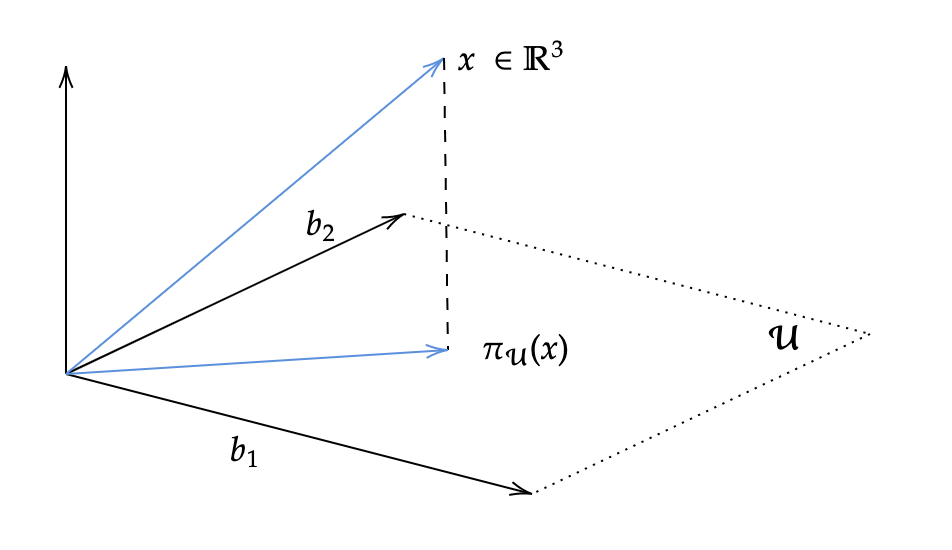
\includegraphics[width=0.5\linewidth]{./resources/projections.png}
    \end{figure}

    The vector $\pi_{\mathcal{U}}(x)$ is the orthogonal projection of vector $x$ onto space $\mathcal{U} = [ b_1, b_2 ]$, where $b_1$ and $b_2$ are the basis that span space $\mathcal{U}$.
    
\end{frame}

\begin{frame}{Projecting Vectors}

    We can represent $\pi_{\mathcal{U}}(x)$ as a linear combination of the basis vectors that span $\mathcal{U}$ since $\pi_{\mathcal{U}}(x) \in \mathcal{U}$.
    \begin{align*}
        \pi_{\mathcal{U}}(x) = \lambda_1 b_1 + \lambda_2 b_2
    \end{align*}

    Moreover, given that the difference vector $x - \pi_{\mathcal{U}}(x)$ is orthogonal to $\mathcal{U}$, its inner product with the basis vectors that span $\mathcal{U}$ must be zero.
    \begin{align*}
        \langle x - \pi_{\mathcal{U}}(x), b_1 \rangle &= 0
        \\
        \langle x - \pi_{\mathcal{U}}(x), b_2 \rangle &= 0
    \end{align*}

    This can be applied to an $M$-dimensional space.
    
\end{frame}

\begin{frame}{Generalizing to $M$-Dimensional Spaces}

    In an $M$-dimensional, define the following:
    \begin{align*}
        \lambda_{M \times 1} =  \begin{bmatrix}
                                    \lambda_1 \\
                                    \vdots \\
                                    \lambda_M \\
                                \end{bmatrix}, \quad
                                B_{D \times M} = \begin{bmatrix} b_1, \cdots, b_M \end{bmatrix}
    \end{align*}

    We can then write the equations we had in the previous slide as:
    \begin{align*}
        \pi_{\mathcal{U}}(x) &= \sum_{i=1}^M \lambda_i b_i
        \\
        \langle x - \pi_{\mathcal{U}}(x), b_i \rangle &= 0, \qquad i=1, \cdots, M
    \end{align*}

    where $x$ now is a $D$-dimensional vector. But as we saw before, we can write the first equation as:
    \begin{align*}
        \pi_{\mathcal{U}}(x) = \sum_{i=1}^M \lambda_i b_i = B \lambda
    \end{align*}
    
\end{frame}

\begin{frame}{Generalizing to $M$-Dimensional Spaces}

    Plug in the matrix representation to get:
    \begin{align*}
        \langle x - B \lambda, b_i \rangle &= 0
    \end{align*}

    The inner product satisfies the linearity property, which means that:
    \begin{align*}
        \langle x - B \lambda, b_i \rangle &= \langle x, b_i \rangle - \langle B \lambda, b_i \rangle= 0
    \end{align*}

    Applying the dot-product as an inner product space we get:
    \begin{align*}
        \langle x, b_i \rangle - \langle B \lambda, b_i \rangle &= 0
        \\
        x^T b_i - \lambda^T B^T b_i &= 0
    \end{align*}

    The last line above can be seen as a set of conditions for all basis $b_i$ in $i = 1, \cdots, M$, which allows us to write it as:
    \begin{align*}
        x^T B - \lambda^T B^T B &= 0_{M \times 1}
    \end{align*}
    
\end{frame}

\begin{frame}{Generalizing to $M$-Dimensional Spaces}

    Remember, we are interested in finding $\lambda$ that allows us to perform the orthogonal projection of an $M$-dimensional vector onto a $D$-dimensional space. We can re-arrange the above and play around with it:
    \begin{align*}
        x^T B - \lambda^T B^T B &= 0_{M \times 1}
        \\
        \lambda^T B^T B &= x^T B
        \\
        \lambda^T &= x^T B (B^T B)^{-1}
        \\
        \lambda &= (B^T B)^{-1} B^T x
    \end{align*}

    where above we use the fact that $(B^T B)^{-1} = [(B^T B)^{-1}]^T$ since $(B^T B)^{-1}$ is a symmetric matrix, so its inverse equals the original matrix. \textbf{Does this look familiar?}
    
\end{frame}

\begin{frame}{Generalizing to $M$-Dimensional Spaces}

    To recap, we said that:
    \begin{align*}
        \pi_{\mathcal{U}}(x) &= B \lambda
        \\
        \lambda &= (B^T B)^{-1} B^T x
    \end{align*}

    Combine the two equations and we have that:
    \begin{align*}
        \pi_{\mathcal{U}}(x) &= \underbrace{B (B^T B)^{-1} B^T}_{\text{projection matrix}} x
    \end{align*}

    So the matrix $B (B^T B)^{-1} B^T$ projects the $M$-dimensional vector $x$ onto the $D$-dimensional space spanned by the basis vectors in $B$.
    
\end{frame}

% Linear algebra section -------------------------------------------------------
% Being section ----------------------------------------------------------------
\section{Coding}

% Tools subsection -------------------------------------------------------------
\subsection{Tools}

\begin{frame}{Useful Tools}
    If you plan on working with data, you must know how to code.
    \begin{itemize}
        \item \textbf{Clean code:} Your code must be easy to understand.
        \item \textbf{Reproducible code:} More and more the profession requires code to be easily reproduced in any system (how can I trust a paper if I cannot replicate it?).
    \end{itemize}

    \vspace{2em}
    
    For most of us, knowing one or two high-level programming languages is enough, but you must know how to use it efficiently.
    \begin{itemize}
        \item \textbf{Efficiency:} Can I make this code run faster?
    \end{itemize}

    Before we dive into R, let's look at some useful results.
    
\end{frame}

% Leverage subsection ----------------------------------------------------------
\subsection{Leverage}

\begin{frame}{Leverage}
    Depending on the data we are working with, we might want to know (probably do) which observations are more or less influential in computing our estimator. Recall that we derived the projection matrix before as:
    \begin{align*}
        P = X(X'X)^{-1}X' =  X(X'X)^{-1}X'Y = X \hat{\beta}
    \end{align*}
    
    We can get the diagonal elements of the projection matrix by looking at the $i$-th observation in matrix $X$ to get
    \begin{align*}
        h_{ii} = x_i (X' X)^{-1} x_i'
    \end{align*}

    Intuitively, this tells us how much the matrix $P$ that projects $Y$ onto the space spanned by the columns of $X$ moves by a given observation. This is often called the leverage

\end{frame}

\begin{frame}{Jackknife}
    Imagine you want to estimate the impact of income on some variable, but you have Mark Zuckerberg as an observation. This will throw off your estimate, so you might want to know what your estimator would be like without that observation.

    \vspace{2em}
    
    You could simply remove it from the data and re-run your OLS, but what if you want to do this for each observation to see how much your estimator change? That's a lot of work. Instead, note that the \href{https://en.wikipedia.org/wiki/Sherman-Morrison_formula}{\underline{Sherman-Morrison formula}} states that for a non-singular matrix $A$ and vector $b$ the following holds:
    \begin{align*}
        (A - bb')^{-1} = A^{-1} + (1 - b'A^{-1}b)^{-1} A^{-1} bb' A^{-1}    
    \end{align*}

\end{frame}

\begin{frame}{Jackknife}
    Using this formula, we know then that:
    \begin{align*}
        (X'X - x_ix_i') &= (X'X)^{-1} + (1 - \underbrace{x_i' (X'X)^{-1} x_i}_{= h_{ii}})^{-1} (X'X)^{-1} x_i x_i' (X'X)^{-1}
    \end{align*}

    We can calculate the \textbf{leave-one-out} estimator by removing observation $i$ from our dataset:
    \begin{align*}
        \hat{\beta}_{-i} = (X'X - x_i x_i')^{-1} (X' Y - x_i y_i)
    \end{align*}

    Plug in the result from the Sherman-Morrison formula (cont.)

\end{frame}

\begin{frame}{Jackknife}
    The leave-one-out estimator can be written as:
    \begin{align*}
        \hat{\beta}_{-i} &= \underbrace{(X'X)^{-1} X' Y}_{= \hat{\beta}} - (X'X)^{-1} x_i y_i
        \\
        &+  (1 -h_{ii})^{-1} (X'X)^{-1} x_i x_i' (X'X)^{-1} (X' Y - x_i y_i)
        \\
        &= \hat{\beta} - (X'X)^{-1} x_i y_i
        \\
        &+ (1 - h_{ii})^{-1} (X' X)^{-1} (x_i x_i' \underbrace{(X'X)^{-1} X' Y}_{= \hat{\beta}} - x_i \underbrace{x_i' (X'X)^{-1} x_i}_{= h_{ii}} y_i)
        \\
        &= \hat{\beta} - (1 - h_{ii}) (X'X)^{-1} x_i \Biggr((1 - h_{ii})y_i - x_i' \hat{\beta} + h_{ii} y_i \Biggr)
        \\
        &= \hat{\beta} - (1 - h_{ii}) (X'X)^{-1} x_i \Biggr(y_i - x_i' \hat{\beta} \Biggr)
    \end{align*}

\end{frame}

\begin{frame}{Jackknife}
    But $y_i - x_i' \hat{\beta}$ is the residual $\hat{e}_i$ of the OLS regression, which then gives the final result
    \begin{align*}
        \hat{\beta}_{-i} &= \hat{\beta} - (X'X)^{-1} x_i \underbrace{(1 - h_{ii}) \hat{e}_i}_{\equiv \tilde{e}_i}
    \end{align*}

    The term $\tilde{e}_i$ is the leave-one-out residual or prediction error. The expression above allows us to see whether $\hat{\beta}$ moves a lot or not if we take observation $i$ out.

    \vspace{2em}

    Importantly, this expression shows us that we don't have to run lots of regressions to get the the estimators we want.

\end{frame}

% Standard errors subsection ---------------------------------------------------
\subsection{Standard errors}

\begin{frame}{OLS Variance}
    Recall that we can calculate the conditional variance of the OLS estimator as follows:
    \begin{align*}
        \operatorname{Var}(\hat{\beta}_{OLS} \mid X) &= \operatorname{Var}\Biggr( (X'X)^{-1} X' Y \mid X \Biggr)
        \\
        &= (X'X)^{-1} X' \operatorname{Var}(Y \mid X) X (X'X)^{-1}
    \end{align*}
    
    But $Y = X \beta + \varepsilon \implies \operatorname{Var}(Y \mid X) = \operatorname{Var}(\epsilon \mid X) = \Omega$, where $\beta$ and $\epsilon$ are the true values. This means we can write the conditional variance of our estimator as:
    \begin{align*}
        \operatorname{Var}(\hat{\beta}_{OLS} \mid X) &= (X'X)^{-1} (X' \Omega X) (X'X)^{-1}
    \end{align*}

    The middle term is simply
    \begin{align*}
        (X' \Omega X) = \sum_{i=1}^n x_i x_i' \sigma_i^2
    \end{align*}
    
\end{frame}

\begin{frame}{OLS Variance}
    If we know the true values of $\varepsilon$, we can use them to calculate the variance:
    \begin{align*}
        \operatorname{Var}(\hat{\beta}_{OLS} \mid X) &= (X'X)^{-1} \Biggr( \sum_{i=1}^n x_i x_i' \varepsilon_i^2 \Biggr) (X'X)^{-1}
    \end{align*}

    This estimator is clearly unbiased:
    \begin{align*}
        \mathbb{E}[\operatorname{Var}(\hat{\beta}_{OLS} \mid X)] &= (X'X)^{-1} \Biggr( \sum_{i=1}^n x_i x_i' \mathbb{E}[\varepsilon_i^2] \Biggr) (X'X)^{-1}
        \\
        &= (X'X)^{-1} \Biggr( \sum_{i=1}^n x_i x_i' \sigma_i^2 \Biggr) (X'X)^{-1}
    \end{align*}

    But we don't really know the true value of $\varepsilon$.
    
\end{frame}

\begin{frame}{Heteroskedasticity Consistent Estimates}
    In R, we have a few options we can use to compute our standard errors:
    \begin{align*}
        \operatorname{Var}(\hat{\beta}_{OLS} \mid X)_{HC0} &= (X'X)^{-1} \Biggr( \sum_{i=1}^n x_i x_i' \hat{e}_i^2 \Biggr) (X'X)^{-1}
        \\
        \operatorname{Var}(\hat{\beta}_{OLS} \mid X)_{HC1} &= (X'X)^{-1} \Biggr( \sum_{i=1}^n x_i x_i' \hat{e}_i^2 \Biggr) (X'X)^{-1} \Biggr( \frac{n}{n-k} \Biggr)
        \\
        \operatorname{Var}(\hat{\beta}_{OLS} \mid X)_{HC2} &= (X'X)^{-1} \Biggr( \sum_{i=1}^n (1 - h_{ii})^{-1} x_i x_i' \hat{e}_i^2 \Biggr) (X'X)^{-1}
        \\
        \operatorname{Var}(\hat{\beta}_{OLS} \mid X)_{HC3} &= (X'X)^{-1} \Biggr( \sum_{i=1}^n (1 - h_{ii})^{-2} x_i x_i' \hat{e}_i^2 \Biggr) (X'X)^{-1}
    \end{align*}

    The last two we compute by summing over the leave-one-out estimates.
    
\end{frame}

% End document -----------------------------------------------------------------
\end{document}